\documentclass[letterpaper]{article}

\usepackage{amsmath}
\usepackage{amssymb}
\usepackage{amsthm}
\usepackage{commath}
\usepackage{enumerate}
\usepackage{lmodern}
\usepackage{microtype}
\usepackage{fullpage}
\usepackage{graphicx}
\usepackage[cache=false]{minted}
\usepackage{hyperref}

\title{STAT 527: Assignment \#3}
\author{Philip Pham}
\date{\today}

\DeclareMathOperator{\E}{E}
\DeclareMathOperator{\Prob}{P}

\begin{document}
\maketitle

\section*{Problem 1}

\begin{enumerate}[(a)]
\item \begin{proof}
    We can rewrite
    \begin{align*}
      \hat{\beta}
      &= \operatorname{argmin}_{\beta \in \mathbb{R}^{k+1}}
        \left(y - Z_{x_0}\beta\right)^\top W_{x_0} \left(y - Z_{x_0}\beta\right),
    \end{align*}
    which is just the weighted least squares problem, so
    \begin{align*}
      \hat{\beta}
      &= \left(Z_{x_0}^\top W_{x_0} Z_{x_0}\right)^{-1}Z_{x_0}^\top W_{x_0}y
    \end{align*}

    Now, we can write $\hat{f}(x_0)$ as
    \begin{align*}
      \hat{f}(x_0)
      &= e_1^\top \hat{\beta} = e_1^\top\left(Z_{x_0}^\top W_{x_0} Z_{x_0}\right)^{-1}Z_{x_0}^\top W_{x_0} y \\
      &= \left(e_1^\top\left(Z_{x_0}^\top W_{x_0} Z_{x_0}\right)^{-1}Z_{x_0}^\top W_{x_0}\right) y,
    \end{align*}
    so can write $s_{x_0}$ as
    \begin{equation}
      s_{x_0} = W_{x_0}Z_{x_0}\left(Z_{x_0}^\top W_{x_0} Z_{x_0}\right)^{-1} e_1
      \label{eqn:sx0}
    \end{equation}

    % \begin{align*}
    %   \hat{f}\left(x_0\right)
    %   &= \frac{\mathbf{1}^\top W_{x_0}Z_{x_0}}{\mathbf{1}^\top W_{x_0}\mathbf{1}}\hat{\beta} \\
    %   &=\sum_{i=1}^n
    %     \hat{\beta_0}
    %     + \sum_{j=1}^k \hat{\beta}_k
    % \end{align*}    
  \end{proof}
\item See Listing \ref{lst:sx0} for a Python implementation. See Figure
  \ref{fig:loess} for the plots of $s_{x_0}$.
  \begin{listing}
    \begin{minted}{python}
import numpy as np
from statsmodels.nonparametric import kernel_regression

def calculate_weights(n, h, k, x0):
    x = np.linspace(1/n, 1, n)
    Z = np.stack([np.power((x - x0)/h, i) for i in range(k + 1)], 1)
    W = np.diag(kernel_regression.kernel_func['gaussian'](h, x, x0))
    return W.dot(Z.dot(np.linalg.inv(Z.T.dot(W).dot(Z))))[:, 0]
  \end{minted}
    \caption{A Python implementation of Equation \ref{eqn:sx0}.}
    \label{lst:sx0}
  \end{listing}

  \begin{figure}
    \caption{Plots of $s_{x_0}$ with various $k$.}
    \centering
    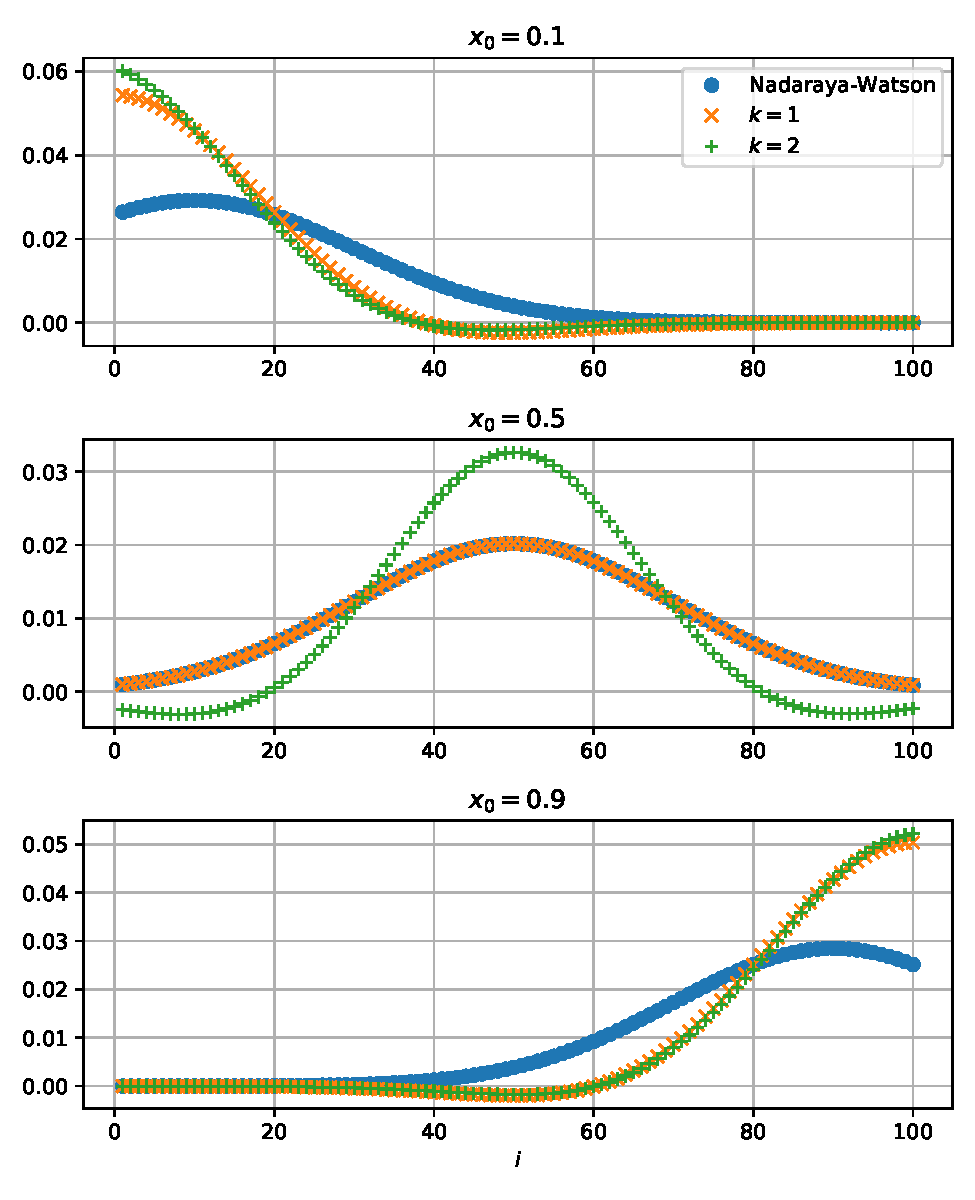
\includegraphics{loess.pdf}
    \label{fig:loess}
  \end{figure}

  In all cases, points observations associated with points near $x_0$ receive
  the most weight. Increasing $k$ appears to more strongly emphasize the local
  neighborhood. The effect is more pronounced at $x_0 = 0.5$ for $k=2$. At the
  tail and head, at $k = 1$ and $k = 2$ do not differ much.
\end{enumerate}

\end{document}
%%% Local Variables:
%%% TeX-command-extra-options: "-shell-escape"
%%% End: